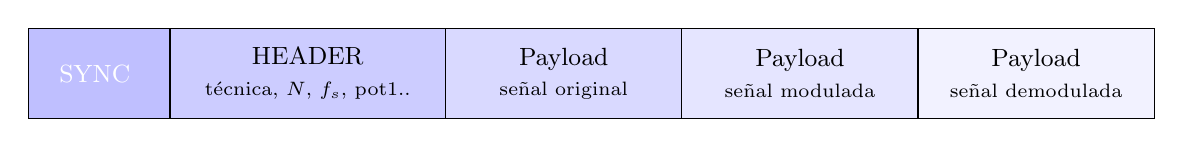
\begin{tikzpicture}[
    font=\small,
    block/.style={
        draw,
        minimum height=1.15cm,
        align=center
    }
]

\node[block, fill=blue!25, text=white, minimum width=1.8cm] (sync) at (0,0) {
SYNC
};

\node[block, fill=blue!20, minimum width=3.5cm] (header) at (2.65,0) {
HEADER\\
\scriptsize técnica, $N$, $f_s$, pot1..
};

\node[block, fill=blue!15, minimum width=3.0cm] (msg) at (5.9,0) {
Payload\\
\scriptsize señal original
};

\node[block, fill=blue!10, minimum width=3.0cm] (mod) at (8.9,0) {
Payload\\
\scriptsize señal modulada
};

\node[block, fill=blue!5, minimum width=3.0cm] (dem) at (11.9,0) {
Payload\\
\scriptsize señal demodulada
};

\end{tikzpicture}